Estudiaremos primero el software GNU Radio, el cual nos permitirá desarrollar prácticas en temas de comunicaciones.

\section{Inicios de la SDR}

En la evolución de las telecomunicaciones inalámbricas han aparecido diversas tecnologías
para el intercambio de información entre dos puntos distantes, con requisitos cada vez más
exigentes. Las incompatibilidades entre las diferentes tecnologías han supuesto un problema a la hora de reutilizar equipos o prestar determinados servicios, como por ejemplo los terminales de telefonía móvil. La SDR surge para solucionar estos inconvenientes de compatibilidad e interoperabilidad, definiendo un conjunto de procedimientos y técnicas orientadas a realizar el procesamiento de señales radio por medio de un dispositivo de propósito general, el cual puede ser modificado mediante software logrando así un cambio dinámico, automático y eficiente entre tecnologías sin tener que incurrir en costes, de ahí surge la necesidad de diseñar un dispositivo capaz de entregar en banda base, o low IF, la señal radio para su procesamiento digital, incluso si la señal es analógica. El dispositivo debe ser configurable para que sea posible recibir distintos anchos de banda y frecuencias para posteriormente, con un procesado digital, poder realizar la sincronización y la detección de la señal recibida.

La primera implementación importante del concepto SDR fue en el proyecto militar estadounidense SpeakEasy, cuyo objetivo era implementar más de 10 tipos de tecnologías de comunicaciones inalámbricas en un equipo programable, operando en la banda de frecuencias de 2MHz a 200MHz. Un objetivo adicional del proyecto era que el prototipo debía tener la posibilidad de actualizar su código para que así se pudieran tener en cuenta los estándares futuros. El proyecto empezó en 1991 y sólo en 1995 fue posible lograr todos los objetivos planteados. El problema fue que únicamente se podía realizar una comunicación a la vez, por lo cual se modificaron sus alcances apareciendo así una segunda fase en la cual se trabajarían

\section{\textit{Wireless Innovation Forum}}

Actualmente no hay ningún estándar sobre SDR, pero sí existe un grupo de trabajo
denominado Wireless Innovation Forum, que es un foro dedicado a conducir la innovación
tecnológica en el campo de la SDR desarrollando estándares y especificaciones del mismo,
logrando así la divulgación de dicha tecnología para soportar necesidades tanto militares y
civiles como comerciales. Los miembros de este grupo constituyen una amplia base en el diseño de plataformas Software Defined Radio (SDR), Cognitive Radio (CR) y Dynamic Spectrum
Acces (DSA). Cuenta con el apoyo de más de 100 empresas, instituciones y organizaciones
como Altera, Xilinx, NASA, VirginiaTech, Toshiba, Samsung, Lockheed, Motorota,
QUALCOMM, Hitachi u Ohio Aerospace Institute, entre otras. El Wireless Innovation Forum
prepara una serie de eventos periódicos en los que se presentan productos, avances y estándares que proponen las empresas inscritas en él con respecto al tema mencionado.

\section{El concepto de SDR}

El concepto SDR ha ido evolucionando con los años pero se siguen basando en el esquema
básico que se muestra en la Figura \ref{cap1:001}, compuesta por tres bloques funcionales: sección de RF, sección de IF y sección Banda Base. La parte de RF e IF se implementan en hardware mientras que la sección de Banda Base en software.

\begin{figure}[htb]
\centering
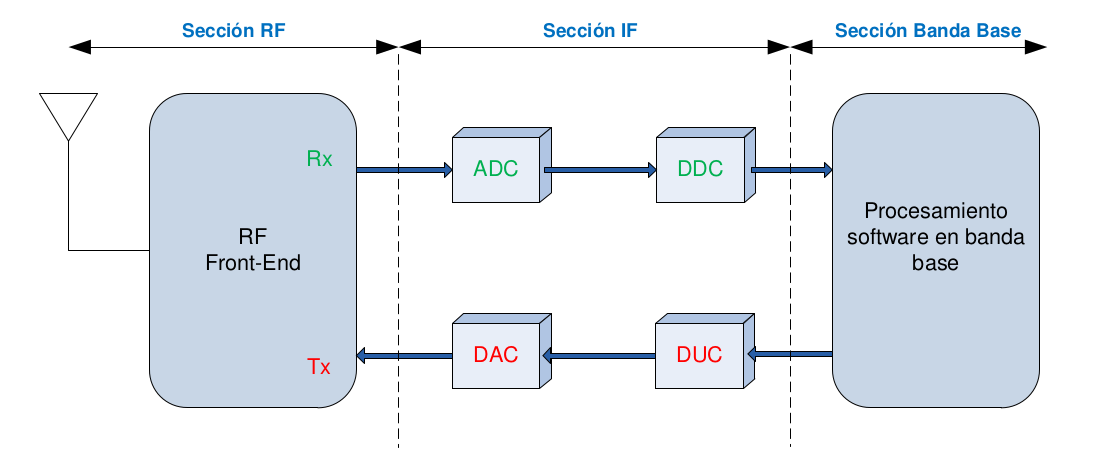
\includegraphics[width=0.6\textwidth]{capitulo1/bloquesSDR.png}
\caption{Diagrama de bloques funcionales del SDR}
\label{cap1:001}
\end{figure}

La sección de RF también denominada RF Front-End es la encargada de transmitir/recibir las
señales de radiofrecuencia para adecuarlas y convertirlas en frecuencia intermedia (IF, intermediate frequency) en recepción o amplificar y modular las señales de IF en el caso de transmisión. La frecuencia intermedia puede ser 0, dando lugar al concepto de Zero-IF; el cual es posible gracias a los avances en los componentes hardware.

De igual manera, la sección de IF se encarga de pasar la señal de IF a banda base y digitalizarla en recepción o pasar la señal de banda base a IF y hacer la conversión digital-analógica de la señal en el caso de la transmisión. Las encargadas de la conversión analógica-digital o digital-analógica de la señal son los módulos ADC/DAC. A su vez, se insertan los módulos DDC/DUC para poder bajar/subir, respectivamente, la tasa de muestreo en el sentido de recepción/transmisión, consiguiendo que la tasa de muestras por la interfaz entre IF y banda base sea inferior.
La sección de Banda Base es la encargada de todo el procesamiento en banda base de la señal como modulación/demodulación, análisis espectral de la señal,.. llevándose a cabo en software.

\section{Aplicaciones de Mercado}

Actualmente, numerosos proyectos de SDR se están llevando a cabo, entre ellos cabe
destacar el ambicioso proyecto OpenBTS con el que se implementa una estación base de
telefonía GSM en software a partir de la arquitectura GNU Radio y el USRP apoyándose en
Asterisk\footnote{Asterisk es un programa de software libre (bajo licencia GPL) que proporciona funcionalidades de
una central telefónica (PBX). Como cualquier PBX, se puede conectar un número determinado
de teléfonos para hacer llamadas entre sí e incluso conectar a un proveedor de VoIP.}  para servicio VoIP. Antes de mostrar la arquitectura funcional, conviene introducir el funcionamiento del USRP con la siguiente figura \ref{cap1:002}.

\begin{figure}[htb]
\centering
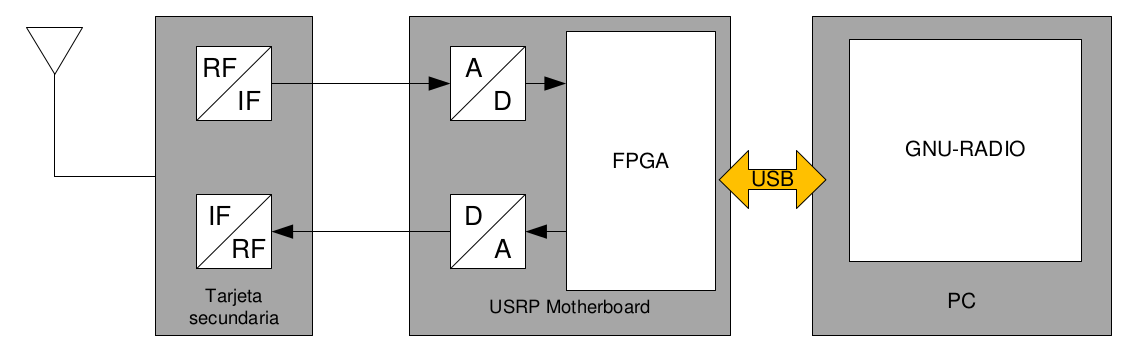
\includegraphics[width=0.6\textwidth]{capitulo1/USRP.png}
\caption{Diagrama básico del \textit{Universal Software Radio Peripheral}}
\label{cap1:002}
\end{figure}

La señal radio es captada o transmitida por la antena y pasando por la tarjeta secundaria. En
la motherboard se produce la conversión A/D y D/A respectivamente y en la FPGA se realiza un
procesado de la señal digital para reducir la tasa de muestras en la interfaz USB. Finalmente se conecta al PC mediante dicha interfaz para realizar el procesamiento software con la arquitectura GNU Radio.
La diagrama funcional del proyecto OpenBTS se muestra en la Figura \ref{cap1:003}.

\begin{figure}[htb]
\centering
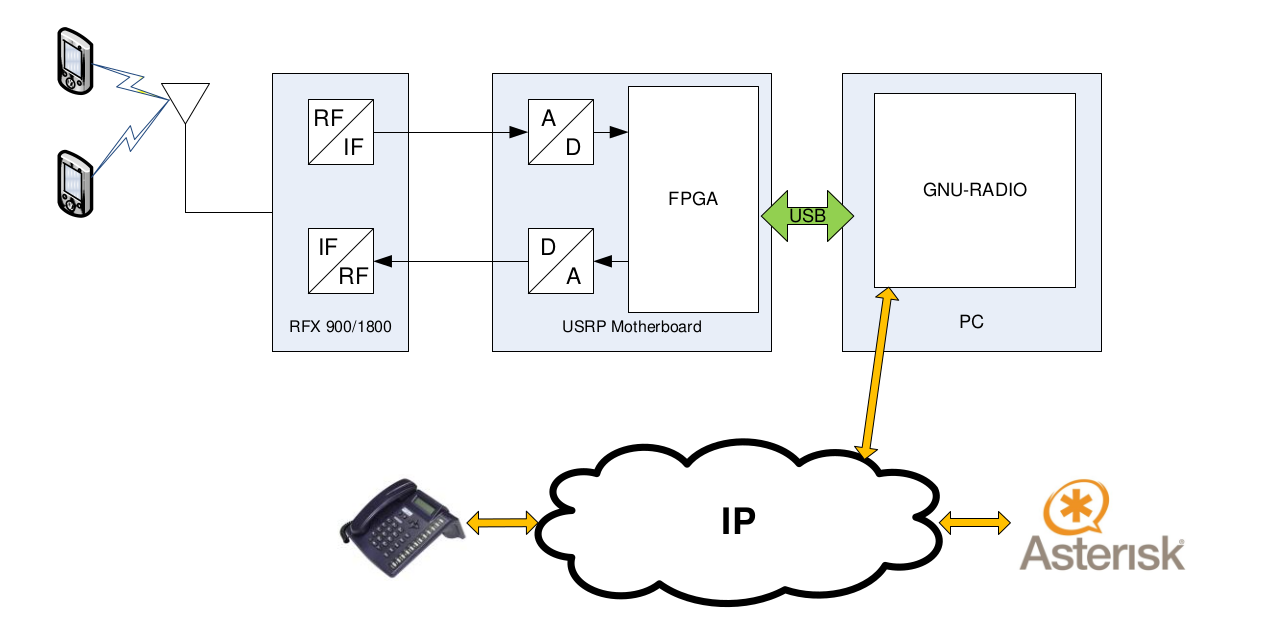
\includegraphics[width=0.6\textwidth]{capitulo1/openBTS.png}
\caption{Arquitectura openBTS}
\label{cap1:003}
\end{figure}



\section{¿Qué es GNU Radio?}

GNU Radio es un software de desarrollo de herramientas de código libre y abierto que proporciona bloques de procesamiento de señales para implementar software radio. Este puede ser usado con hardware de RF externo de bajo costo para crear radios definidos por software o sin hardware utilizando el entorno de simulación. Es ampliamente utilizado en entornos de aficionados, académicos y comercial para contribuir tanto en la investigación de comunicaciones inalámbricas y sistemas de radio del mundo real.
GNU Radio está licenciado bajo la GNU General Public License (GPL) versión 3. Todo el código es propiedad de la Fundación del Software Libre.
Las aplicaciones de GNU Radio son escritas a principio utilizando el lenguaje de programación Python, mientras que el suministro de herramientas críticas de procesamiento de señales que requieren alto rendimiento son implementados en C++ usando extensiones de procesamiento de punto flotante, cuando este esta disponible. Así, el desarrollador es capaz de implementar, de manera simple, sistemas de radio de alto rendimiento funcionando a tiempo real aprovechando el ambiente de desarrollo de aplicaciones de manera inmediata.

Aunque no es una herramienta principalmente de simulación, GNU Radio complementa el desarrollo de algoritmos de procesamiento de señales a partir de datos previamente grabados o generados, evitando la necesidad de hardware de RF.

GNU Radio está licenciado bajo el GNU General Public License (GPL) versión 3. Todo el código es propiedad de la Fundación del Software Libre.

GNU Radio es un conjunto de archivos y aplicaciones agrupadas en librerías, que permiten
manipular señales radio mediante procesado digital de señales. Mediante estas librerías se
realiza el diseño de sistemas radio definidos por software si se conecta el PC/Workstation a un SDR, aunque también se puede trabajar con la tarjeta de audio por ejemplo. GNU Radio corre sobre sistemas operativos (SO) GNU/Linux como Ubuntu. También es posible la instalación en Mac y Windows, algo más complejo en éste último SO utilizando la herramienta Cygwin, cuyo objetivo es portar software de sistemas POSIX \footnote{POSIX es el acrónimo de Portable Operating System Interface; la X viene de UNIX como seña de identidad de la API. Son una familia de estándares de llamadas al sistema operativo definidos por el IEEE.
Persiguen generalizar las interfaces de los sistemas operativos para que una misma aplicación pueda ejecutarse en distintas plataformas.}  a Windows.
Los diseños realizados en GNU Radio se programan en Python. Python es un lenguaje de
programación interpretado, es decir, no se compila sino que el sistema operativo ejecuta
directamente, interactivo y orientado a objetos. Habitualmente se compara a TCL, Perl, Scheme, Java y Ruby. Cabe decir que, además de realizar diseños en Python, es posible utilizar la aplicación GNU Radio Companion. GNU Radio Companion es una herramienta que mediante una interfaz gráfica basada en bloques, similar a Simulink en Matlab, facilita la labor de diseño, creando los ficheros Python a partir del esquemático que se cree, tal y como se verá en apartados posteriores.
Actualmente, Python se desarrolla como un proyecto de código abierto, administrado por la
Python Software Foundation. Contiene módulos, clases, tipos de datos de alto nivel y escritura dinámica. Tiene interfaces para diversos sistemas y librerías. También puede utilizarse como un lenguaje de extensión para aplicaciones que necesitan una interfaz programable. Otra ventaja es su portabilidad, funcionando en sistemas Unix y derivados, Windows, Dos, Mac y otros.
Para construir un sistema de radio con GNU Radio se debe crear un grafo, donde los nodos
son bloques de procesado de señal y los enlaces entre nodos representan el flujo de datos entre ellos. Los bloques de procesado de señal son implementados en C++ y portados a Python a partir del programa SWIG, es decir, para implementar los diseños se crearán los módulos en
Python que a su vez se apoya en los bloques implementados en C++. Las interacciones entre
los diferentes niveles de GNU Radio aparecen en la siguiente figura:

\begin{figure}[htb]
\centering
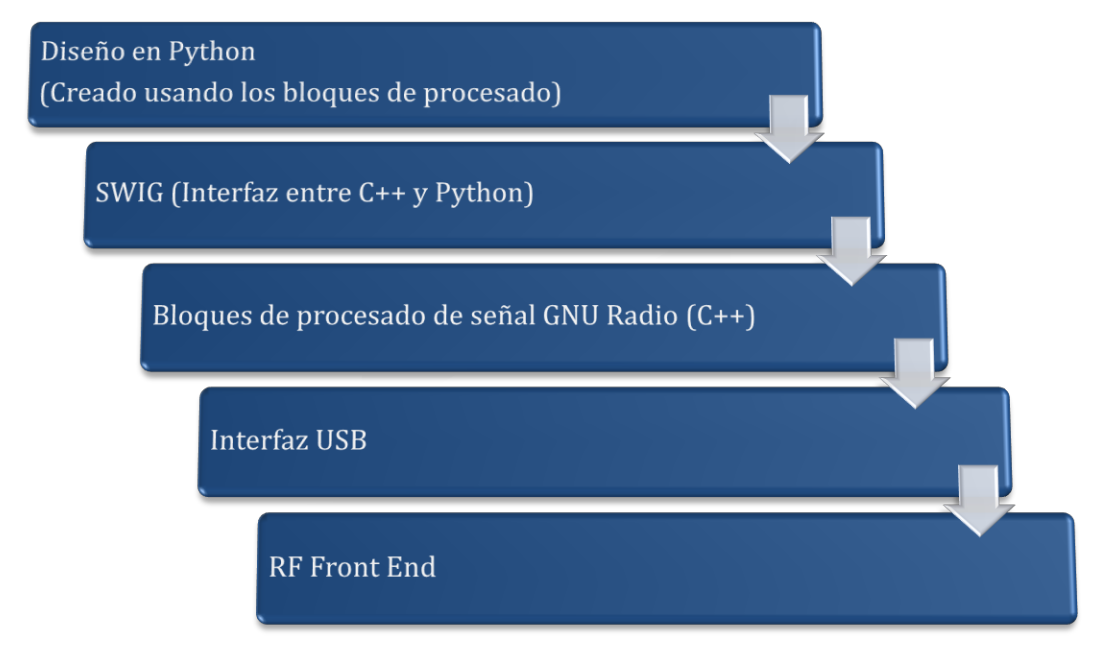
\includegraphics[width=0.6\textwidth]{capitulo1/ArqGNURadio.png}
\caption{Arquitectura GNU Radio}
\label{cap1:004}
\end{figure}

Conceptualmente un bloque procesa señales, de forma continua, desde puertos de entrada
hasta puertos de salida. Las partes de un bloque son el número de puerto de entrada, el número del puerto de salida, y el tipo de dato que fluirá de uno al otro. Los tipos de datos más comunes son: ``short'', ``float'', ``complex'' y ``byte''.
Algunos bloques tienen únicamente puertos de salida o puertos de entrada. Éstos sirven como
fuente de datos y señales en una gráfica por ejemplo. Existen fuentes que leen datos de un
archivo o de la FPGA a través de la interfaz USB, y señales que escriben datos a un archivo, a la FPGA, a la tarjeta de audio o a un display gráfico.

\section{Gráficos de flujo y ¿de qué están hechos?}

Antes de ir a ninguna parte, primero debemos comprender los conceptos más básicos sobre GNU Radio: gráficos de flujo y bloques.

Los gráficos de flujo son gráficos (como en la teoría de gráficos) a través de los cuales fluyen los datos. Muchas aplicaciones de GNU Radio no contienen nada más que un diagrama de flujo. Los nodos de dicho gráfico se denominan bloques y los datos fluyen a lo largo de los bordes.

Cualquier procesamiento de señal real se realiza en los bloques. Idealmente, cada bloque hace exactamente un trabajo, de esta manera GNU Radio permanece modular y flexible. Los bloques generalmente se escriben en C ++ (también podría ser Python); escribir nuevos bloques no es muy difícil.

Para aclarar un poco este tema difuso, comencemos con un ejemplo (todos estos ejemplos fueron creados con GNU Radio companion (GRC), una interfaz gráfica de usuario para GNU Radio).

Aquí tenemos tres bloques (los rectángulos). Los datos fluyen de izquierda a derecha en este ejemplo, lo que significa que se originan en la fuente de audio, pasan a través del filtro de paso bajo y terminan en un archivo que se escribe en el disco duro.



Los bloques están conectados en puertos. El primer bloque no tiene puerto de entrada, produce muestras. Tal bloque, con solo puertos de salida, se llama fuente. De manera analógica, el bloque final, sin salidas, se llama sumidero.

A veces, esto es confuso: desde la perspectiva del usuario, el bloque de audio (que toma muestras de la tarjeta de sonido) es solo una parte del procesamiento. Cuando hablamos de sumideros y fuentes, siempre nos referimos a la perspectiva del diagrama de flujo.

Entonces, ¿qué está pasando aquí? El bloque de fuente de audio está conectado al controlador de la tarjeta de sonido y emite muestras de audio. Estas muestras están conectadas al filtro de paso bajo, que las procesa más. Finalmente, las muestras se pasan a un bloque que las escribe en un archivo WAV.

\section{Diseño de módulos de GNU Radio}

La creación de módulos en Python puede llevarse a cabo de dos formas: bien programando
directamente en Python o bien utilizando la herramienta GNU Radio Companion. La
programación en Python es ardua, mientras que el diseño basado en GNU Radio Companion es
más sencillo. De ahí que los diseños de este documento se centren en esta herramienta. El lector interesado en la programación en Python encontrará interesante el Anexo III, donde se introduce a la programación en este lenguaje. GNU Radio Companion es una herramienta gráfica para realizar un diseño a partir de bloques incluidos en librerías o creados por el usuario. Una vez realizado el diseño, el GNU Radio Companion genera el código en Python asociado, que
bien puede ejecutarse desde la propia herramienta o desde la línea de comandos en un terminal.

Para aquellos que sean usuarios de Matlab, cabe decir que la filosofía de funcionamiento es
similar a la de Simulink. El GNU Radio Companion permite diseñar sistemas que utilicen un SDR como el USRP, pero también permite trabajar con, por ejemplo, las señales de audio del PC/Workstation.

Para iniciarnos en la programación de Software Radio con GNU Radio Companion es
necesario conocer y saber cómo funcionan las estructuras de grafos, bloques y conexiones.

La construcción de módulos utilizando esta herramienta gráfica se basa en añadir bloques e
interconectarlos de manera esquemática 6 . Los bloques utilizados se pueden agrupar de la
siguiente manera:

\section{Instalación}

Para la instalación de GNU Radio se recomienda utilizar la versión binaria que viene la la distribución de linux, en este caso se ocupa el comando:

\begin{lstlisting}
$ sudo apt-get install gnuradio
\end{lstlisting}

La primera pantalla al ejecutar GNU Radio es la que se indica en la figura \ref{cap1:004}.

\begin{figure}[htb]
	\centering
	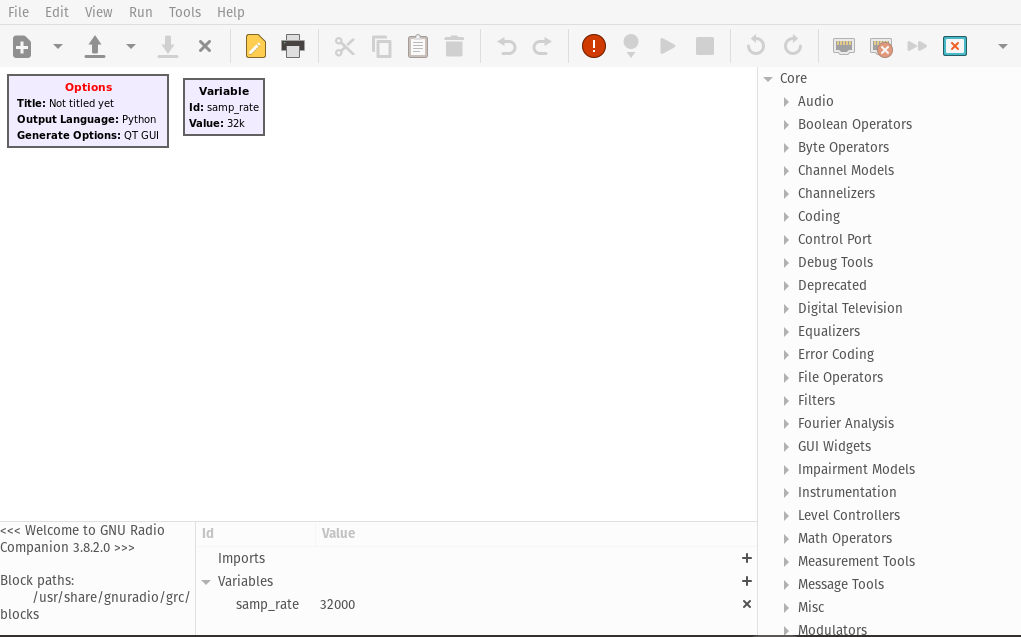
\includegraphics[width=0.6\textwidth]{capitulo1/primerapantalla.png}
	\caption{Primera pantalla de GNU Radio}
	\label{cap1:004}
\end{figure}

Como se podrá notar el bloque \textbf{Options} esta en color rojo indicando que hay datos incorrectos que deben ser corregido. Si pulsamos dos veces en el bloque, obtenemos la pantalla que se muestra en la figura \ref{cap1:005}.

\begin{figure}[htb]
	\centering
	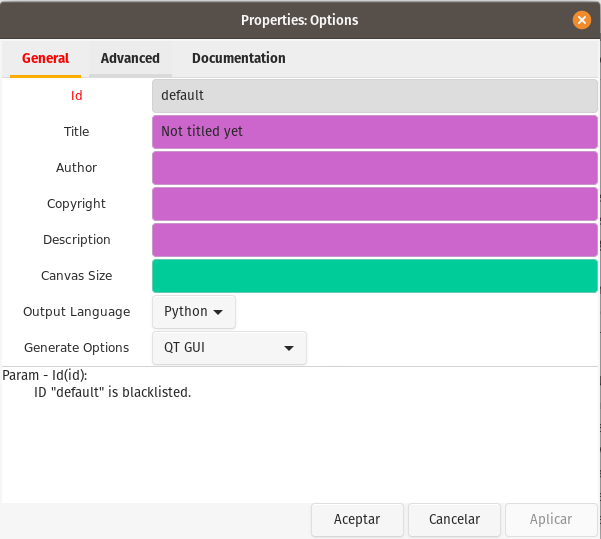
\includegraphics[width=0.6\textwidth]{capitulo1/datosgenerales.png}
	\caption{Datos generales a llenar para el proyecto}
	\label{cap1:005}
\end{figure}

De la figura llenamos los datos solicitados, es importante señalar que el error del bloque se elimina cuando cambiamos el ID del proyecto por uno único e irrepetible.

\section{Ejemplo 1: Modulación AM}

Se inicia el análisis de la modulación sobre la Ecuación \ref{equ:1001}, la cual se relacionará nuevamente a continuación.


\begin{equ}[!ht]
  \begin{equation}
    v(t) = V cos(2 \pi f t + \theta)
  \end{equation}
\caption{Ecuación de una señal senoidal}
\label{equ:1001}
\end{equ}

Las modulaciones análogas se desarrollan haciendo uso de dos señales
principales, la de información y la portadora. Por consiguiente, la modulación AM
produce el cambio en amplitud de la señal portadora con respecto a la señal de
información. Teniendo en cuenta lo anterior, se muestra el proceso matemático
mediante el cual se genera la ecuación de una señal AM para todo tiempo t. Se considera la fase $\theta = 0$, debido a que la modulación altera los valores de amplitud
de las expresiones y el cambio de la fase es indiferente para el desarrollo del
procedimiento de modulación por amplitud. Entonces, siendo:

\begin{equ}[!ht]
  \begin{equation}
    v_{c}(t) = V_{c} cos(2 \pi f_{c} t )
  \end{equation}
\caption{Ecuación de una señal portadora}
\label{equ:1002}
\end{equ}

La ecuación \ref{equ:1003} para la señal de información:

\begin{equ}[!ht]
  \begin{equation}
    v_{m}(t) = V_{m} cos(2 \pi f_{m} t )
  \end{equation}
\caption{Ecuación de una señal de información}
\label{equ:1003}
\end{equ}

la señal modulada en amplitud será el resultado del valor pico de la señal portadora en adición al valor instantáneo de la señal de información. Entonces se tiene:

\begin{equ}[!ht]
  \begin{equation}
    \begin{array}{cr}
		v_{AM}(t) = (V_{c} + v_{m}(t))sin(2 \pi f_{c} t) \\
		v_{AM}(t) = (V_{c} + V_{m}sin(2 \pi f_{m} t))sin(2 \pi f_{c} t) \\
		v_{AM}(t) = V_{c}(1 + \frac{V_{m}}{V_{c}}sin(2 \pi f_{m} t))sin(2 \pi f_{c} t) \\
	\end{array}
  \end{equation}
\caption{Ecuación de una señal de información}
\label{equ:1004}
\end{equ}


